\section{Architektur}
Grundsätzlich lassen sich zwei unterschiedliche Architekturansätze im Bereich Data Streaming unterscheiden:

\begin{description}
\item [Lambda Architektur:] Benannt nach dem griechischen ($\lambda$) zeichnet sich dieser Ansatz dadurch aus, dass die Streaming Daten zweigleisig verarbeitet werden. Zum einen wird der Datenstrom direkt in einen häufig auf In-Memory Technologie basierenden \textit{Speed Layer} geleitet, der diese in Echtzeit verarbeitet und dem \textit{Serving Layer} zur Verfügung stellt. Da Streams per Definition unendlich und der Speed Layer teuer und physikalisch endlich ist, wird der Stream von \textit{Ingestion Layer} parallel in den \textit{Batch Layer} geleitet. Dieser speichert zunächst die Daten persistent und startet nach einem fest definierten Intervall einen Batch-Job um die bis dahin angelaufenen Daten zu verarbeiten und zum Serving Layer zu übertragen. Es ist also die nicht zu unterschätzende  Verantwortung des Serving Layers, die aggregierten Bestandsdaten aus dem Batch Layer mit den Echtzeitdaten des Speed Layers, die noch nicht vom Batch Layer verarbeitet worden sind, abzumischen.

\begin{figure}[h]
	\centering
	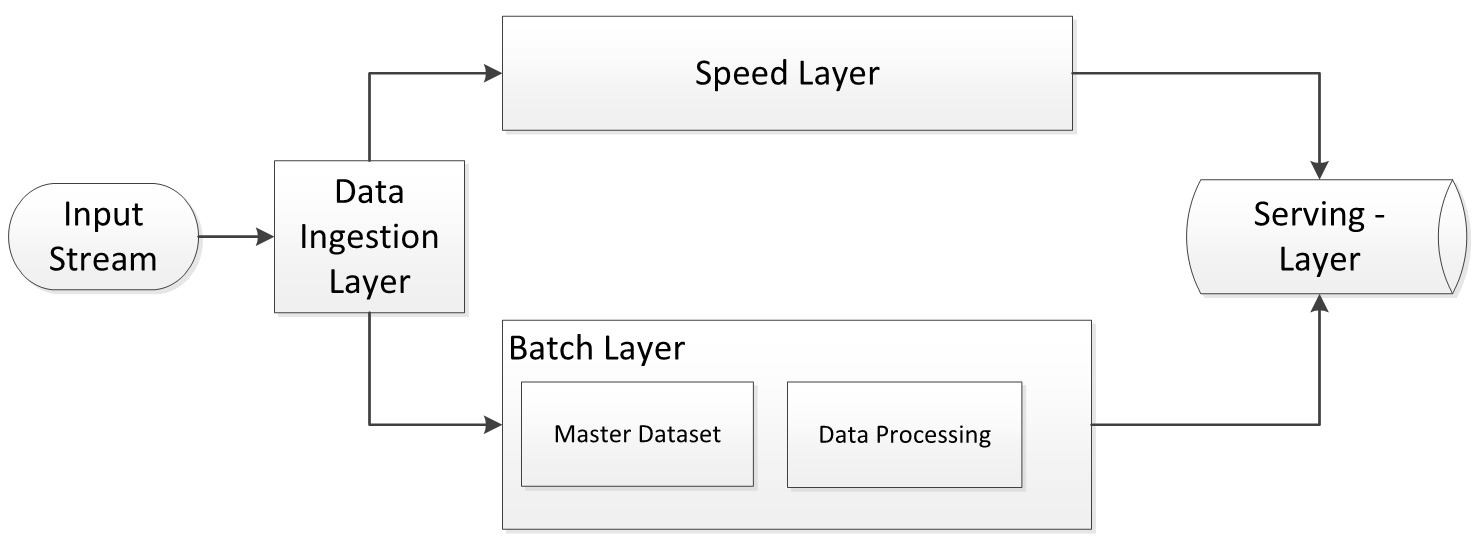
\includegraphics[width=10cm]{berle_lambda-architektur_3.jpg}
	\caption[Schema der $\lambda$ Architektur]{Schema der $\lambda$ Architektur\citep{TODO}}
	\label{fig:KafkaArchitecture}
\end{figure}
 

\item [Kappa Architektur:] 

\end{description}



%Warum Kappa? Daten sind endlich aber ausreichend für unsere Bedürfnisse.Haben eh nur Pseudostream.


%https://www.confluent.io/blog/simplest-useful-kafka-connect-data-pipeline-world-thereabouts-part-1/

